\documentclass{article}
\usepackage[utf8]{inputenc}
\usepackage[T1]{fontenc}
\usepackage{polski}
\usepackage{fancyhdr}
\usepackage{indentfirst}
\usepackage{lastpage}
\usepackage{setspace}
\usepackage{longtable}
\usepackage{graphicx}

\setlength{\parskip}{1ex plus 0.5ex minus 0.2ex}

\pagestyle{fancy}
\title{Specyfikacja implementacyjna projektu indywidualnego \textit{,,Bieszczadzki Komiwojażer''}}

\begin{document}
\begin{titlepage}
\makeatletter
\noindent
\vspace{25pt}
\begin{center}
\Large\textsc{\@title}
\end{center}
\makeatother
\vspace{300pt}
\begin{flushright}
\noindent Wykonał: Piotr Ferdynus\\
Sprawdził: mgr inż. Paweł Zawadzki\\
Data: 13.11.2019\\
\end{flushright}


\thispagestyle{empty}
\end{titlepage}

\rhead{Piotr Ferdynus 299244}
\lhead{}
\cfoot{\thepage \hspace{1pt} / \pageref{LastPage}}
\setcounter{page}{2}

\section{Wprowadzenie}

Celem specyfikacji jest sprecyzowanie sposobu implementacji funkcjonalności projektu \textit{,,Bieszczadzki Komiwojażer''}. W dokumencie zostanie określona logika działania programu, opisane zostaną planowane struktury danych oraz zastosowane algorytmy.


\section{Środowisko deweloperskie}
Opis charakterystyki sprzętu i oprogramowania, które zostaną użyte podczas pracy nad projektem.

\subsection{Parametry sprzętowe}
Podczas procesu wytwarzania oprogramowania zostaną wykorzystane dwie stacje robocze o następującej specyfikacji:

    Mobilna stacja robocza:
\vspace{-8pt}    
\begin{verbatim}
        Procesor AMD Ryzen 5 2500U
        Zintegrowana karta graficzna Radeon Vega 8 Mobile
        Pamięć RAM DDR4 8GB
        Windows 10 Home wersja 1903
\end{verbatim}    

    Stacjonarna stacja robocza:
\vspace{-8pt}        
\begin{verbatim}
        Procesor Intel Core i5-7400
        Karta graficzna NVidia Geforce GTX 1060 3GB
        Pamięć RAM DDR4 8GB
        Windows 10 Education wersja 1903
\end{verbatim}

\subsection{Oprogramowanie}

Na obu komputerach zostało zainstalowane oprogramowanie pozwalające na pracę w języku programowania Java:

\begin{verbatim}
    SDK Java 11.0.2 2019-01-15 LTS
    Java(TM) SE Runtime Environment 18.9
    Java HotSpot(TM) 64-Bit Server VM 18.9
    IDE Intellij IDEA Ultimate 2019.1.1 
\end{verbatim}

\section{Przebieg wprowadzania zmian}
Ustalenie sposobu wprowadzania zmian do projektu.

\subsection{Wiadomości do repozytorium}
Komentarze zmian wprowadzanych do repozytorium będą realizować szablon: numer wersji + krótki komentarz. Szczegółowy opis numeru wersji znajduje się w sekcji \textit{Numer wersji}.

\subsection{Numer wersji}
Podczas realizacji projektu zostały przyjęte ogólnie akceptowane zasady wersjonowania projektów informatycznych. Numer wersji występuje w postaci \textit{X.Y.Z}, gdzie X, Y i Z reprezentują liczby naturalne. Człon \textit{X}, indeksowany od zera, to iteracja wydań niekompatybilnych wstecznie lub wnoszących istotne zmiany w funkcjonalności oprogramowania. Człon \textit{Y}, indeksowany od jedynki, reprezentuje mniejszy przyrost funkcjonalności aplikacji. Ostatnia część \textit{Z}, indeksowana od zera, informuje o poprawie błędów w funkcjonowaniu programu.

\subsection{Organizacja repozytorium}
Repozytorium będzie składać się z gałęzi \textit{master} i \textit{dev}. Główna gałąź (\textit{master}) będzie zawierała stabilną, działającą wersję projektu. Wszelkie zmiany i nowe funkcjonalności bedą rozwijane w gałęzi \textit{dev}. Po poprawnym zaimplementowaniu określonej funkcjonalności i uzyskaniu kolejnej iteracji programu, zostanie dokonany merge gałęzi głównej z gałęzią \textit{dev}.

\section{Struktura klas programu}
Przedstawienie i opis planowanego schematu klas gotowego programu oraz przewidywany sposób działania algorytmu.

\subsection{Schemat klas}

\begin{center}
    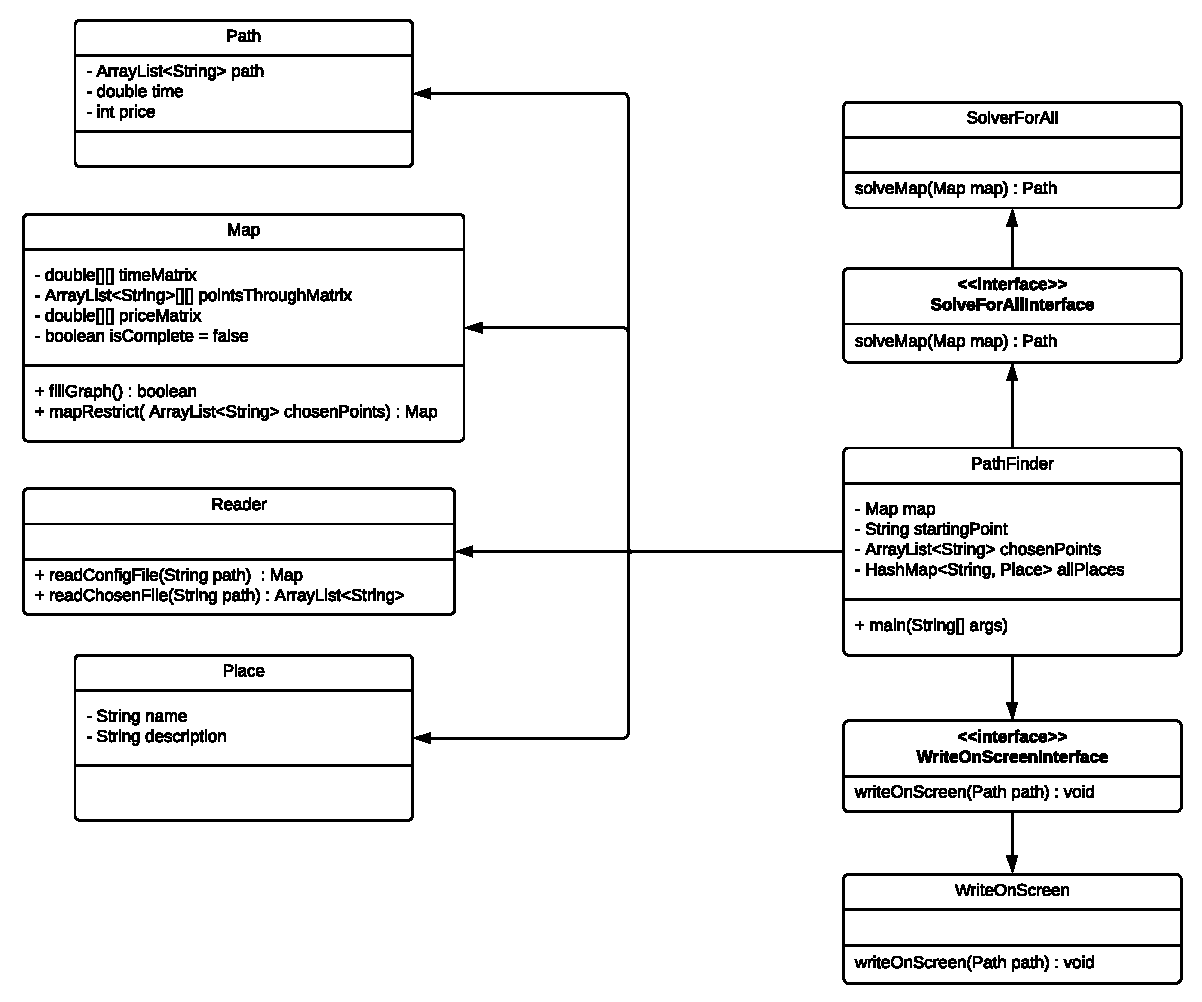
\includegraphics [height=9cm]{diagram_klas.pdf} \newline
    \textit{Diagram klas ,,Bieszczadzki Komiwojażer''}
\end{center}

\subsection{Opis klas}
Przedstawienie funkcji i zadań poszczególnych klas.

\subsubsection{PathFinder}
Klasa głowna, odpowiadająca za obsługiwanie programu. Przyjmuje argumenty wywołania, zarządza przebiegiem rozwiązywania zadanego problemu i komunikacją z użytkownikiem.

\subsubsection{SolverForAll}
Klasa odpowiada za właściwe wyznaczenie rozwiązania. Szczegółowy opis działania klasy i zastosowanych w niej algorytmów znajduje się w części \textit{Schemat działania} i \textit{Algorytmy}.

\subsubsection{Path}
Klasa umożliwiająca ustrukturyzowane przechowywanie wyznaczonej optymalnej ścieżki.

\subsubsection{Map}
Klasa odpowiadająca za przechowywanie danych o mapie Bieszczad i wykonywanie najważniejszych operacji. Wczytane punkty i trasy je łączące zostaną zapisane w postaci macierzy incydencji grafu skierowanego \textit{timeMatrix}, w której w odpowiednich indeksach zostanie zawarta długość trasy pomiędzy punktami według następującego schematu:

\begin{center}
    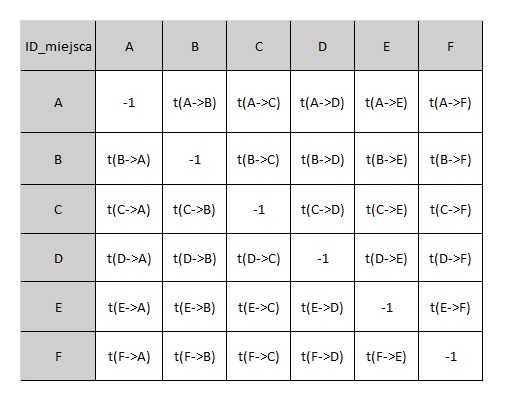
\includegraphics[height=8cm]{timeMatrix.jpg} \\
    \textit{Schemat macierzy timeMatrix po wczytaniu danych}
\end{center}

Jeżeli dwa wierzchołki nie są połączone krawędzią, wartość przechowywana w macierzy wynosi \textit{-1}. Analogicznie uzupełniana jest macierz \textit{priceMatrix}, w której przechowywane wartości odzwierciedlają wysokość opłaty na konkretnym odcinku trasy.

Metoda \textit{fillGraph} jest kluczowa dla działania programu. Wykorzystując algorytm Djikstry, opisany w sekcji \textit{Algorytmy}, uzupełnia ona brakujące krawędzie grafu, wyznaczając najkrótszą drogę pomiędzy wierzchołkami. Jeżeli najkrótsza droga przebiega przez inne wierzchołki, zostają one zapisane w postaci listy liniowej w odpowiednim polu macierzy \textit{pointsThroughMatrix}. 

Metoda \textit{mapRestrict} ogranicza mapę tak, by zawierała jedynie te wierzchołki, których \textit{ID\_miejsca} znajduje się w liście \textit{chosenPoints}.

\subsubsection{Reader}
Klasa odpowiadająca za prawidłowe odczytanie danych z plików wejściowych oraz o odpowiednie zakomunikowanie o występujących w nich błędach. Metody \textit{readConfigFile()} i \textit{readChosenFile()} są odpowiedzialne za, odpowiednio, odczyt pliku konfiguracyjnego i odczyt pliku z wybranymi miejscami.

\subsubsection{Place}
Klasa pozwalająca na przechowywanie danych o miejscach odczytanych z pliku.

\subsubsection{WriteOnScreen}
Klasa wypisująca wynik końcowy.

\subsection{Schemat działania}
Klasa \textit{PathFinder} rozpoczyna analizę argumentów wejściowych. Inicjalizuje odczyt plików wywołując odpowiednie metody klasy \textit{reader}. Następnie wywołuje metodę \textit{fillGraph()} klasy \textit{Map}. Szczegółowy opis działania tej metody znajduje się w sekcji \textit{Opis klas}. Jeżeli został podany plik zawierający wybrane miejsca, wywołuje metodę \textit{mapRestrict()}. Tak przygotowane dane zostają przekazane do funkcji \textit{solveMap()}. Otrzymany obiekt typu \textit{Path} zostaje przekazany do metody \textit{showPath} i wypisany w sposób zrozumiały dla użytkownika.

\section{Algorytmy}
Podczas rozwiązywania zadanego problemu program będzie korzystał z implementacji następujących algorytmów.

\subsection{Algorytm Djikstry}

\subsubsection{Opis}
Algorytm służy do znajdowania najkrótszej możliwej drogi pomiędzy wybranym wierzchołkiem a pozostałymi wierzchołkami grafu
\subsubsection{Zastosowanie}
Algorytm zostanie zastosowany w metodzie \textit{fillGraph} klasy \textit{Map}, by dopełnić brakujące krawędzie grafu, zastępując je najkrótszą możliwą drogą wiodącą przez jak najmniejszą ilość punktów. 

\subsubsection{Złożoność}
Złożoność czasowa algorytmu w przypadku implementacji przez kopiec to O(E logV), gdzie E reprezentuje liczbę krawędzi, a V liczbę wierzchołków.

\subsection{Algorytm Helda-Karpa}

\subsubsection{Opis}
Algorytm służy do znajdowania minimalnego drzewa rozpinającego dla grafu pełnego, to jest drzewa łączącego wszystkie wierzchołki grafu o najmniejszej sumie wag. Wzór algorytmu ma postać rekurencyjną i przedstawia się następująco:\\
$$
\left\{ \begin{array}{ll}
D(S, p) = d_{1,p} & \textrm{gdy $s=1$}\\
D(S, p) = min_{x \in (S-{p})}( D(S-{p}, x) + d_{x,p}). & \textrm{gdy $s>1$}\\
\end{array} \right.
$$
    
S -- zbiór wierzchołków grafu
    
p $\in$ S -- wierzchołek grafu na którym ma zakończyć się droga
    
D(S, p) -- najkrótsza możliwa droga z wybranego wierzchołka początkowego, przez wszystkie wierzchołki ze zbioru S, kończąca się na wierzchołku p.

\subsubsection{Zastosowanie}
W programie zostanie wykorzystany do wyznaczenia najkrótszej możliwej drogi zawierającej wszystkie wierzchołki w grafie.

\subsubsection{Złożoność}
    Złożoność czasowa algorytmu wynosi O(n$^{2}2^{n}$).


\section{Struktury danych}
Opis wykorzystanych struktur danych i cel ich zastosowania.

\subsection{Kopiec}
    Kopiec zostanie wykorzystany do implementacji kolejki priorytetowej, niezbędnej przy implementacji algorytmu Djikstry, opisanego w sekcji \textit{Algorytmy}.
    
\subsection{Macierz}
    Macierz zostanie wykorzystana do przechowywania informacji o mapie wczytanej do programu.
    
\subsection{Tablica mieszająca}
    Tablica mieszająca (z ang. \textit{hash table}) zostanie wykorzystana do przechowywanie szczegółowych danych na temat punktów, jako klucz wykorzystując ich \textit{ID\_miejsca}.

\subsection{Lista liniowa}
    Lista liniowa w postaci \textit{ArrayList<>} zostanie wykorzystana do przechowywania listy wybranych miejsc.

\end{document}